\documentclass{cls/styleMemoireCeFri}

 \typeMemoire{DIPLOME DE LICENCE EN INFORMATIQUE GÉNÉRALE}
 \etudiant{\textbf{AROUNA} Hospice Alfred }
 \titreDuMemoire{Solution libre de supervision réseau: initialisation automatique du NAV en utilisant SNMP}
 \dateSoutenance{Le jeudi 20 décembre 2012}
 \promo{2\up{ème}}
 \annee{2011-2012}

 %maitre de mémoire
 \encadrant{Monsieur Toussaint OKEY}

 %Jury
 % President
 \juryP{\textbf{Président} : Dr \textbf{ADEDJOUMA} Semiyou A., Enseignant-Chercheur à l'EPAC}
 %Liste des membres 
 \juryMembre{\textbf{Membres} :}
 %Premier rapporteur
 \juryR{1°) Dr. \textbf{Baloïtcha} Ezinvi, Coordonnateur des études au CEFRI}
 %Examinateur
 \juryE{2°) Mme \textbf{Gnonlonfoun} Miranda, Enseignant au CEFRI}
 %second rapporteur
 \juryRa{~}
 %second examinateur
 \juryEx{~}

 %Paramètres du fichier PDF
 \hypersetup{
 pdftitle={Solution libre de supervision r\'eseaux: initialisation automatique du NAV en utilisant SNMP},
 pdfauthor={Hospice Alfred AROUNA, aang@arouna.net},
 pdfsubject={Supervision des grands r\'eseaux avec une solution libre bas\'ee sur SNMP},
 pdfkeywords={r\'eseau, supervision, monitoring, SNMP, client, serveur, CeFRI} 
 }

 %Couleur grise
 \color{bookColor}
  
 \begin{document}
  
   %%%% Début Préambule %%%%
    %Page de titre
    \pageTitre
  
    %Page blanche pour la page de garde
  	\pagecolor{white}
  
  	%Page vide
  	\thispagestyle{empty}\ \clearpage
  
  	%Page du jury
  	\pageJury
  
  	%Page blanche pour le reste du document
  	\pagecolor{white}
 
  	%Sommaire
  	%Numérotation romaine
  	\pagenumbering{roman}

  	%Inclure le glossaire avant les appels et dans la TOC
  	
\newacronym{qos}{QoS}{Quality of Service}
\newacronym{tcp}{TCP}{Transmission-Control Protocol}
\newacronym{ip}{IP}{Internet Protocol}
\newacronym{udp}{UDP}{User Datagram Protocol}
\newacronym{osi}{OSI}{Open Systems Interconnection}
\newacronym{iso}{ISO}{International Standard Organization}

\newacronym{snmp}{SNMP}{Simple Network Management Protocol}
\newacronym{cmip}{CMIP}{Common Information Management Protocol}
\newacronym{lan}{LAN}{Local Area Network}
\newacronym{wan}{WAN}{Wide Area Network}
\newacronym{tmn}{TMN}{Telecommunication Management network}
\newacronym{ieee}{IEEE}{Institute of Electrical and Electronics Engineers}

\newglossaryentry{supervision}
{
name=Supervision,
description={
Superviser consiste à indiquer/modifier l'état d'un système informatique ou d'un hôte. La supervision  est donc la fonction qui permet de remonter/éditer les informations techniques relatives à un hôte ou a un ou des réseaux. En d'autres termes, la supervision de réseaux peut être définie comme l'utilisation de ressources réseaux (matériel et logiciel) adaptées dans le but d'obtenir des informations (en temps réel ou non) sur l'utilisation ou la condition des hôtes dans le réseau  afin d'assurer un niveau de service garanti, une bonne qualité et une répartition optimale et de ceux-ci.}
}

\newglossaryentry{typologie}
{
name=Typologie,
description={
La topologie d'un réseau peut se définir comme l'étude de la structure du réseau et des interconnexion entre hôtes. La typologie réseau peut être de type \emph{link layer topology}, \emph{network layer topology} ou \emph{Internet topology} et \emph{overlay topology}.}
}

\newglossaryentry{seeddb}
{
name=seedDB,
description={
L'étape du \emph{Seed Database} permet de fournir les informations importantes pour NAV pour pouvoir parcourir et découvrir le réseau. En effet, après installation et démarrage de NAV, NAV ne fait rien si les paramètres n'ont pas été fournis à la base.}
}

\newglossaryentry{agent}
{
name=Agent (SNMP),
description={Composant logiciel ou matériel qui gère les MIBs d'un matériel. Les agents répondent aux requêtes du Manager ou lui envoie un trap en cas d'alerte.}
}

\newglossaryentry{trap}
{
name=Trap,
description={Message d'alerte (problème qui nécessite une attention) envoyé par un agent au manager suite à un incident.}
}

\newglossaryentry{manager}
{
name=Manager,
description={Le manager est l'élément actif de la supervision. Il collecte les informations des hôtes en interrogeant les agents. Il reçoit aussi les traps provenant des agents. }
}

\newglossaryentry{standard}
{
name=Standard,
description={Un standard est une norme, un modèle à suivre. Dans le contexte des RFCs, un standard est le statut d'une proposition de norme, après les états de \emph{proposed} et \emph{draft}}.
}

\newglossaryentry{netkit}
{
name=NetKit,
description={Netkit permet de créer plusieurs  machines virtuelles sur le même hôte. Chaque machine virtuelle est reliée à un ou des domaines de collisions virtuels permettant ainsi les communications entre-elles. Chaque machine virtuelle peut jouer le rôle de PC, routeur ou switch.}
}

\newacronym{sgmp}{SGMP}{Simple Gateway Management Protocol}
\newacronym{asn}{ASN.1}{Abstract Syntax Notation .1}
\newacronym{ber}{BER}{Basic Encoding Rules}
\newacronym{mib}{MIB}{Management Information Base}
\newacronym{oid}{OID}{Object IDentifier}
\newacronym{nms}{NMS}{Network Management System}
\newacronym{smi}{SMI}{Structure of Management Information}
\newacronym{rfc}{RFC}{Request for Comments}
\newacronym{ietf}{IETF}{Internet Engineering Task Force}
\newacronym{itu}{ITU}{International Telecommunication Union}

\newacronym{sha}{SHA}{Secure Hash Algorithm}

\newacronym{pdu}{PDU}{Protocol Data Unit}
\newacronym{md5}{MD5}{Message Digest 5}
\newacronym{des}{DES}{Data Encryption Standard}
\newacronym{usm}{USM}{User-based Security Model}
\newacronym{vacm}{VACM}{View Access Control Model}

\newacronym{mac}{MAC}{Media Access Control}
\newacronym{icmp}{ICMP}{Internet Control Message Protocol}
\newacronym{egp}{EGP}{Exterior Gateway Protocol}
\newacronym{aes}{AES}{Advanced Encryption Standard}
\newacronym{popi}{POP}{Point Of Presence}
\newacronym{as}{AS}{Autonomous System}
\newacronym{dns}{DNS}{Domain Name System}

\newacronym{gpl}{GPL}{Global Public Licence}
\newacronym{nav}{NAV}{Network Administration Visualized}
\newacronym{noc}{NOC}{Network Operation Center}
\newacronym{acl}{ACL}{Access List Control}
\newacronym{iana}{IANA}{Internet Assigned Numbers Authority}
\addcontentsline{toc}{chapter}{Glossaire}
  
  	%Résumé
  	\selectlanguage{french}
  	\resume
\begin{abstract}
L'assurance de la qualité de service (\emph{\gls*{qos}}) fournie aux utilisateurs est un élément primordial dans la gestion des réseaux. Cette assurance de la qualité de service est possible grâce à la \gls*{supervision} qui permet d'être actif et surtout d'être pro-actif. \textbf{La supervision permet de résoudre les problèmes du réseau avant qu'ils ne surviennent, et même en cas de problème, de pouvoir avoir la bonne information (source du problème) et de prendre la meilleure solution.}

La présente étude porte sur notre solution à une des faiblesses d'une application de supervision: le \emph{\gls*{nav}}. \textbf{Notre apport est une implémentation en python des études les majeures relatives à la découverte automatique des équipements et de la \gls*{typologie} d'un réseau en utilisant le standard \emph{\gls*{snmp}}}. Cette implémentation permet un début d'automatisation de l'initialisation de la base de données des équipements du réseau géré par le\emph{\gls*{nav}}: l'étape du \texttt{\emph{\gls*{seeddb}}} se trouve essentiellement simplifiée.

\paragraph{}
\textbf{Mots clés}: \emph{SNMP}, \emph{supervision}, \emph{NAV}, \emph{python}, \emph{réseau}, \emph{sécurité}, \emph{logiciel libre}.
\end{abstract}

\selectlanguage{english}
\begin{abstract}
Ensuring the Quality of Service (\emph{\gls*{qos}}) provided to users is an essential criteria in network management. Monitoring is the main base to have correct QoS. Monitoring allow network administrator to be active and especially to be pro-active. \textbf{Monitoring can help to solve network problems before they occur, and even if something goes wrong,  to be able to get the right and accurate information (root cause of the problem) and take the best solution}.

The present study focuses on our solution to one of the weakness of one monitoring application: \emph{\gls*{nav}}. \textbf{We provided an implementation in python of the most important studies on the automatic discovery of network topology using the standard \emph{\gls*{snmp}} }. This implementation introduce the automation of initializing the database  of network devices managed by the NAV: the step of \texttt{\emph{\gls*{seeddb}}} is essentially simplified.

\paragraph{}
\textbf{Key words}: \emph{SNMP}, \emph{monitoring}, \emph{NAV}, \emph{python}, \emph{network}, \emph{security}, \emph{free software}.
\end{abstract}

  	%Langue française pour la table des matières
  	\selectlanguage{french}
  	\tableofcontents
  
  	%Liste des algo (en français)
  	\selectlanguage{french}
  	\listofalgorithms

  	%Liste des figures
  	\listoffigures 

  	%Liste des tableaux
  	\listoftables

  	%Afficher le glossaire
  	\printglossaries

  	%Remerciements
  	\remerciements

Nos premiers remerciements vont à l'endroit notre encadreur: Mr. Toussaint OKEY, enseignant au Centre de Formation et de Recherches en Informatique (CeFRI); pour sa disponibilité et ses fructueuses orientations.
\paragraph{}
Nos remerciements s'adresse aussi Mr Musa BALTA, du Computer Engineering Department, Faculty of Computer and Information Science du Sakarya Üniversitesi en Turkie. Mr Musa BALTA est l'auteur de l'article \emph{The Discovery of Enterprise Network Topology Created in a Virtual Environment with SNMPv3} paru dans le \emph{TOJSAT: The Online Journal of Science and Technology} d'Avril 2012. Aussi Mr Musa BALTA; suite à notre demande,  a mis gracieusement à notre disposition l'article \emph{SNMP-based enterprise IP network topology discovery} de Pandey et. al. Cet article est la référence actuelle en matière de découverte de la topologie d'un réseau en utilisant \emph{SNMP}.
\paragraph{}

Avant de finir, nous tenons à reconnaitre la qualité de l'enseignement reçue et à remercier toute l'administration de CeFRI.
\paragraph{}
Nous ne saurions finir sans remercier les membres du jury pour l'importance à nous accorder pour l'évaluation de notre travail.

  	\clearpage
  	
  %%%% Fin Préambule %%%%
  
  %%%% Début du document %%%%
  
  	%Numérotation arabe
  	\pagenumbering{arabic}
  	%Numérotation à partir de 1
	\setcounter{page}{1}
	
	%Cacher les entêtes et pieds de pages pour l'introduction
	\lhead[]{} \rhead[]{} \chead[]{}
	%Introduction
	\introduction
Une entreprise moderne dépend d'un réseau informatique dont la taille est dans une croissance permanente. Il est primordial pour cette entreprise de garantir une qualité de service à travers son réseau informatique. C'est dans cette perspective qu'est apparu, il y a maintenant une vingtaine d'années, le concept de supervision de réseau.

Que ce soit le grand réseau d'un opérateur ou d'une université ou bien le petit réseau local d'une petite entreprise, la supervision
doit pouvoir apporter des outils performants, adaptables aussi bien à la taille des réseaux qu'à leur grande diversité technologique.

D'un point de vue pragmatique, la supervision réseau a pour objectif :
\begin{itemize}
\item La \textbf{Pro-Activité} pour anticiper sur les problèmes.
\item La \textbf{Réactivité} suite à un incident.
\item La \textbf{Localisation d'un problème} afin de prendre la meilleure décision.
\end{itemize}


Un des éléments clé de la supervision réseau est la possibilité d'avoir un œil sur le réseau. Quel que soit le type d'administrateur (expérimenté ou non), la vue graphique ou topologie du réseau donne un outil clair et facile pour un début d'analyse du réseau. 

Vu l'importance de la mise à disposition des administrateurs de la typologie du réseau, de nombreuses études ont porté sur la question ; certaines en utilisant  le  \emph{standard}\footnote{Cycle des statuts des RFC: \emph{proposed}, \emph{draft} puis \emph{standard}. Si un RCF a été mis à jour par un autre son statut devient \emph{historical}. De même si un RFC n'est pas encore accepté comme standard, il reste à l'état de \emph{experimental}.} \emph{\gls*{snmp}}. Nous porterons notre attention sur les études portant sur la détection de la typologie au sein d'une organisation.

\emph{\gls*{snmp}} est de nos jours le \emph{standard} de supervision. Crée dans le but de superviser les premiers routeurs lors de l'explosion d'Internet, \emph{\gls*{snmp}} a connu diverses versions pour en être depuis 1999, à la version 3. \emph{\gls*{snmp}} présente les caractéristiques suivantes:
\begin{figure}[H]
    \begin{center}
     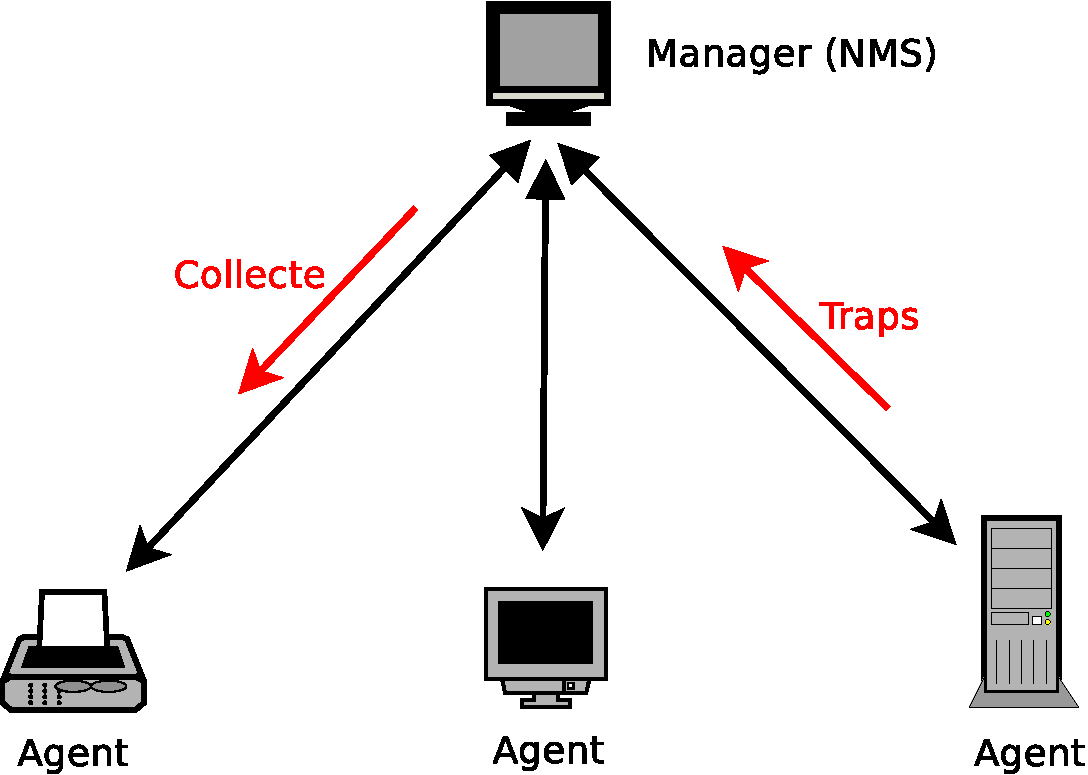
\includegraphics[scale=0.4]{images/snmp_principe.pdf}
     \caption{Mode de fonctionnement de SNMP. \label {fig:snmp}} 
    \end{center}
   \end{figure} 

\begin{itemize}
\item Fonctionne de manière asymétrique:  \emph{\gls*{agent}} et  \emph{\gls*{manager}} (\gls*{rfc} 1157).
\item Utilise des opérations en écriture (\texttt{set}) et en lecture (\texttt{get}).
\item Utilise \texttt{UDP} et le  \emph{\gls*{ber}} pour le transport.
\item Introduit le concept de  \emph{\gls*{mib}} (RCF 1213).
\item Identifie chaque \texttt{MIB} par son  \emph{\gls*{oid}}. 
\end{itemize}



Le présent mémoire porte  de manière générale sur l'implémentation en python de la découverte des équipements d'un réseau d'une organisation en utilisant \emph{\gls*{snmp}}. Cette découverte automatique des équipements du réseau servira de source d'importation des informations sur les équipements du réseau dans une solution libre de supervision: le \emph{\gls*{nav}}.

Le présent document se résume à notre apport pour l'\emph{initialisation automatique de la base de données} du \emph{\gls*{nav}}. Il est composé de deux chapitres:

\paragraph{Présentation théorique de la solution\\}

Le premier chapitre présente brièvement le \emph{\gls*{nav}}. \emph{\gls*{nav}} intègre bien d'autres solutions libres dont les plus importants sont Cricket, PostgreSQL, OpenStreeMap. Ce chapitre se termine sur le présentation de quelques limites du NAV disponible sur la feuille de route du projet. En particulier, l'accent est mis sur la fonctionnalité de l'\emph{autodiscovery-wizard}. Cette fonctionnalité permettra de fournir de manière automatique au NAV la base de données des équipements du réseau. Un début d'implémentation de cette fonctionnalité est donnée dans le cinquième chapitre.

\paragraph{Initialisation automatique de la base de données\\}
Le dernier chapitre constitue notre apport pour l'implémentation de l'\emph{autodiscovery-wizard}. Cette implémentation permet l'\emph{initialisation automatique de la base de données} du NAV. Plus besoin d'ajouter un à un les équipements du réseau ou bien de les lister soi-même dans un fichier. Notre solution en s'inspirant des études en matière de découverte de réseau sur la base de \emph{SNMP} permet de découvrir tous les équipements du réseau et de créer un fichier prêt pour importation dans la base de données du NAV. Après une présentation des algorithmes, l'implémentation en code python est expliquée, suivie des tests et résultats dans un environnement virtuel grâce à  \emph{\gls*{netkit}}.


	%Reafficher les entêtes et pieds de page
	\fancyhead[L]{\tiny \leftmark}
	\fancyhead[R]{\scriptsize \rightmark}
	\fancyfoot[C]{\thepage}
	
	%Premier Chapitre
	\chapter{Le Network Administration Visualized}
		%Première section
    	\section{Présentation rapide}
Le \textbf{Network Administration Visualized} est une suite logicielle de pointe pour superviser les réseaux informatiques de grande taille.

\texttt{NAV} présente les caractéristiques suivantes:

\begin{itemize}
\item Originaire de la Norvège: \emph{NTNU (Norvegian University of Science and Technology)}.
\item Licence GPL v2. 
\item Sous la responsabilité du \emph{UNINETT (the Norvegian research network)}. 
\item Utilisation par de nombreuses universités dans le monde. 
\item Programmation en Python.
\end{itemize}

\paragraph{Intérêt du NAV\\}
\texttt{NAV} est une collection intégrée de solutions libres ayant déjà fait leurs preuves. Ce qui fait de \texttt{NAV}, la seule solution distribuée offrant de nombreuses fonctionnalités.


\paragraph{}
Comme fonctionnalités majeures du \texttt{NAV}, nous avons:
\begin{itemize}
\item \emph{Geographical Map}: typologie sur une carte \emph{OpenStreetMap}.
\item \emph{Network Weather Map}: état d'utilisation des liens (topologie).
\item \emph{Machine Tracker}: historique du couple adresse IP et adresse MAC pour chaque équipement.
\item \emph{Mac Watch}: surveillance des adresses MAC du réseau. 
\item \emph{Layer 2 trace}: trace du parcours d'un paquet d'une source à une destination.
\item \emph{Arnold}: blocage des ports des routeurs et switchs en les mettant en quarantaine.
\item \emph{Maintenance Tasks}: Exclusion d'un équipement du mécanisme de supervision sans enlever l'équipement du réseau.
\item \emph{Radius Accounting}: Suivi à la trace des utilisateurs nomades.
\end{itemize} 



\paragraph{}
Plus d'informations sont disponibles sur le wiki\footnote{\url{http://nav.uninett.no/navtechdoc}} du projet.
    	%Seconde section
    	\section{Limites de NAV}
\subsection{Domaines d'utilisation}
NAV est certes une suite logicielle de pointe pour superviser les réseaux informatiques de grande taille mais NAV ne peut \emph{évidement} pas tout faire.

En effet, NAV est une solution de supervision réseau et non de \emph{configuration} réseau; et ceci à deux exceptions près:
\begin{itemize}
\item L'utilisation de SNMP pour bloquer les ports avec l'outil \emph{Arnlod}.
\item L'utilisation de SNMP pour configurer les ports des switchs et les Vlans avec l'outil \emph{PortAdmin}
\end{itemize}

NAV n'est pas non plus une solution magique qui va découvrir \emph{tous} les problèmes dans le réseau. NAV essaie de découvrir tous les problèmes \emph{importants} sur le réseau et non tous les problèmes. Il s'en va dire que d'autres outils doivent être utilisé pour découvrir ces problèmes. L'exemple classique est celui du statut des équipements. La minute ou la seconde après la vérification du statut de l'équipement par NAV, ce dernier peut changer de statut. Avant la prochaine vérification par NAV, l'équipement peut revenir à son état originel. Ce changement d'état ne sera pas détecter par le NAV.

Aussi NAV ne donne pas des solutions  toutes faites aux problèmes découverts. NAV ne donne que des alertes et des pistes de recherche de solution. D'autres outils d'investigation doivent être utilisés pour trouver la cause fondamentale du problème et ainsi apporter la meilleure solution.


\subsection{Fonctionnalités}
NAV donne des informations sur la charge du trafic, pas sur le sens du trafic, ni les détails sur le trafic (http, ftp, etc). En d'autres termes, NAV ne permet pas de connaître la source, ni la destination d'un paquet comme les sites les plus visités par exemple. D'autres outils libres tels \emph{Netflow Sensor (NfSen)}\footnote{\url{http://nfsen.sourceforge.net/}} le font déjà correctement. Une documentation sur l'usage de Netflow est donné par \emph{The Swiss Education \& Research Network}\footnote{\url{http://meetings.ripe.net/ripe-50/presentations/ripe50-plenary-tue-nfsen-nfdump.pdf}}

NAV à certes de nombreuses fonctionnalités mais de l'avis même de ses concepteurs, il reste encore de nombreuse fonctionnalités potentielles à ajouter au NAV. La liste complète de ses fonctionnalités est disponible sur le \emph{launchpad}\footnote{\url{https://blueprints.launchpad.net/nav}}.

En autre fonctionnalité, NAV ne fait pas au premier abord de la découverte du réseau. Après installation de NAV, il faut initialiser la base de données en y ajoutant les équipements du réseau: c'est l'étape du \emph{seedDB}.

Une automatisation de cette étape permettrait de simplifier l'utilisation du NAV: Il suffirait d'installer NAV; de lancer le script de découverte puis deux minutes après avoir l'état du réseau.

Nous nous proposons dans le chapitre suivant de donner un début de simplification de l'étape du seedDb.
    
    %Second Chapitre	
    \chapter{Initialisation automatique de la base de données}\label{init_db}
    	%Première section
    	\section{Initialisation automatique de la base de données grâce à SNMP}
\monBloc{L'initialisation automatique de la base de données grâce à SNMP constitue notre apport. En effet, avec le modèle actuel proposé par NAV, il faudra actuellement soit ajouter un à un les équipements du réseau, soit remplir un formulaire où chaque ligne correspond à chaque équipement au niveau de l'interface d'administration. Cette tâche s'avère très fastidieuse d'où la nécessité de l'automatiser.}

C'est dans cette perspective que la fonctionnalité \emph{Autodiscovery wizard for NAV} a été prévu sur la feuille de route des futurs développements\footnote{\url{https://blueprints.launchpad.net/nav/+spec/autodiscovery-wizard}}


Nous proposons d'écrire un script permettant de découvrir tous les hôtes du réseau supportant SNMP à partir d'un point de départ. Une fois ces hôtes découvert, il faudra les mettre sous un format acceptable par NAV et les insérer dans la base de données.


\subsection{Études relatives à la découverte de la typologie réseau avec SNMP}
De nombreux études ont porté sur la découverte de la topologie physique et logique des réseaux informatiques. Nous ne citerons ici que les quatre dernières études en la matière:
\begin{enumerate}
\item Pandey S, Choi M, Lee S, Hong J. \footnote{
Suman Pandey, Mi-Jung Choi, Sung-Joo Lee, James W. Hong	Dept. of Computer Science and Engineering, POSTECH, Korea}.\emph{IP Network Topology Discovery Using SNMP}. International Conference on Information Networking (ICOIN'09). 23 33-37 2009 %\cite{AT1}
\item Yang Xiao. \emph{Physical Path Tracing for IP Traffic using SNMP}. BBC Research White Paper WHP 188. 2010 %\cite{AT2}
\item Pandey S, Choi M, Won Y, Hong J. \emph{SNMP-based enterprise IP network topology discovery. International Journal of Network Management} 21 (3) 169-184. 2011 %\cite{AT3}
\item Musa Balta, Ibrahim Özçelik. \emph{The Discovery of Enterprise Network Topology Created in a Virtual Environment with SNMPv3}. The Online Journal of Science and Technology (TOJSAT) Volume 2, Issue 2, 64-70, Avril 2012. %\cite{AT4}
\end{enumerate}
Toutes les trois dernières études se basent sur les résultats de la première étude de la liste ci-dessus: l'étude sur \emph{IP Network Topology Discovery Using SNMP}. 

De ces études, la typologie réseau découverte est de type physique et logique soit le \emph{link layer topology} et le \emph{router level} du \emph{Internet topology} d'une organisation ou d'un AS. C'est donc une découverte de réseau interne à une organisation ou un AS.

La typologie d'un réseau désigne l'organisation des éléments (équipements et liens) du réseau et les interactions physiques et logiques entre ces divers éléments.

La typologie logique se réfère à la structuration ou division logique du réseau en sous réseaux. %Suivant la logique de division considérée, on peut avoir plusieurs typologies logiques pour un même réseau (cas des switchs L2, L3, L4, L5 ou L7).

La typologie physique désigne les communications ou connexions visibles entre hôtes sur des ports grâce à des liens (de transmission).

Dans le cadre de l'automatisation de l'initialisation de la base de NAV, nous n'implémenterons que certains aspects des résultats de ces études. En effet, la fonctionnalité offerte par le \texttt{ipdevpoll} permettent déjà de faire de la mise à jour des informations dans la base. Notre apport permettra de faire des insertions en masse des informations minimales sur chaque équipent découvert dans le réseau.

%\begin{table}[h]
%\begin{center}
% \begin{tabular}{|l|p{3cm}|p{3cm}|p{3cm}|p{3cm}|p{3cm}|}
% \hline
%  & Siamwalla et al.(1999) &  Lowekamp et al.(2001) & Breitbart et al.(2004) & Nazir (2007) & Pandey et al. (2011)\\\hline
%  Method & Ping/broadcast
%   ping/traceroute/
%   zone transfer
%   DSN server/
%   SNMP/subnet
%   guessing algorithm & SNMP & SNMP (ICMP
%  spoofing/
%  heuristics)
%& SNMP/ping & Only SNMP
%
% \\\hline
%
%\end{tabular}
%\caption{Comparaison des méthodes de découverte de la typologie réseau} \label{comparaison_typologie_réseau}
%\end{center}
%\end{table}


    	%Seconde section
   		\section{Les algorithmes}
Se basant sur les études citées dans la section précédente, nous proposons un algorithme pour initialiser la base de données conformément au \emph{minimum requirement} c'est-à-dire le \emph{Level 1: Minimum requirements}\footnote{\url{http://nav.uninett.no/seedessentials}} du \emph{seed database}.


L'algorithme proposé par Pandey and et. al. (2011) se déroule en étapes successives:

\begin{verbatim}
1. Take network information inputs
2. Device discovery
       a. Device discovery using next hop mechanism
       b. Device discovery using ARP cache entries
3. Device type discovery
4. Device grouping based on IP address
5. Connectivity discovery
       a. L2 to L2 connectivity
       b. L2 to L3 connectivity
       c. L3 to L3 connectivity
       d. L2 and L3 to end host connectivity
6. Subnet discovery and connectivity discovery in subnet
7. VLAN discovery and connectivity discovery in VLAN

\end{verbatim}



Un projet d'algorithme est aussi précisé sur la page du wiki\footnote{\url{http://metanav.uninett.no/devel:blueprints:autodiscovery-wizard}}.

La  première étape est la récupération des paramètres nécessaires pour la découverte des hôtes du réseau. Comme paramètres proposés nous avons:
\begin{itemize}
\item La \emph{communauté SNMP} pour l'accès en  lecture des MIBs.
\item Un préfixe ou une liste des préfixes (plage d'adresses IP de la découverte réseau).
\item L'adresse IP du routeur de départ.
\item Le nom de l'organisation auquel appartient les adresses IP (les équipements).
\end{itemize}
Une fois les paramètres donnés au script, les étapes suivantes sont proposées:


\begin{verbatim}
1. Retrieve all active arp records 
2. For each of these IP addresses
    a. If the IP address exists in NAV - skip
    b. Tf the address answers to SNMP : new device found!
    c. Get system.syslocation
    d. Set orgid to the supplied orgid
    e. Decide category
    f. Make new row to bulk file (format: roomid:ip:orgid:catid:ro )
\end{verbatim}

\paragraph{Notre algorithme est une mise en commun des quatre premières étapes proposées par Pandey and et. al. (2011) et de l'algorithme proposé pour la fonctionnalité de découverte des équipements du réseau. Nous ne prenons pas en compte la découverte de la connectivité (topologie)  et des VLAN. \texttt{ipdevpoll} s'occupe déjà de ces deux dernières fonctionnalités dans NAV. \\}

Notre algorithme de découverte du réseau se présente en six étapes suivantes:
\begin{verbatim}
1. Starting Point (Take network information inputs)
2. Device discovery
       a. Device discovery using next hop mechanism
       b. Device discovery using ARP cache entries
3. Device grouping based on IP address
4. Device type discovery
5. Create Bulk format
	   a. Set default roomid.
	   b. Set default orgid
	   c. Set category (type discovery)
	   d. Make new row to bulk file (format: roomid:ip:orgid:catid:ro )
6. Store in Db
\end{verbatim}
%a. If the IP address exists in NAV - skip
%b. Call bulk function to save in DB
%La dernière étape correspond essentiellement l'étape 2 de l'algorithme proposé par Vidar Faltinsen.


\subsection{Starting Point}
{\fontfamily{phv}\selectfont
\begin{center}
\begin{algorithm}
\caption{Starting Point}
\label{starting_point}

\begin{algorithmic}[1]
\Require $R\_IP \gets Starting ~ router~ IP~for ~ network~ discovery$
\Require $V\_SNMP \gets SNMP~ version$
\Require $C\_SNMP ~ community~ or~ security~ parameters~$
\Ensure $boolean \gets Router ~ SNMP~ availability~$

\Function{Starting\_Point}{$R\_IP,V\_SNMP,C\_SNMP$}
   \If{$R\_IP~ is~ manageable $}
    \State \Return $True$
   \Else
    \State \Return $False$
   \EndIf
    
\EndFunction

\end{algorithmic}

\end{algorithm}
\end{center}
}
Avec le mode de fonctionnement asymétrique de \emph{SNMP},   \emph{\gls*{agent}} et  \emph{\gls*{manager}} utilisent comme protocole de transport l' \emph{\gls*{udp}}.\\
Or \emph{UDP} (couche 4) se base sur le protocole  \emph{\gls*{ip}} (couche 3). Le critère de base de  fonctionnement de \emph{SNMP} est donc la présence dans le réseau d'équipement à même de supporter \emph{UDP} et par conséquent \emph{IP}. De manière plus simple, il faut que les équipements  membres du  \emph{\gls*{nms}} possèdent une adresse \emph{IP} valide.\\
La découverte d'un équipement du réseau repose donc sur ce critère de base: les équipements en communication doivent avoir chacun une adresse IP valide. L'adresse IP du \textbf{routeur} spécifié est considérée comme adresse source (algorithme \ref{starting_point}, page \pageref{starting_point}). Si le routeur ne supporte pas SNMP ou ne répond pas correctement à la requête SNMP (Community invalide), le processus de découverte s'arrête. Dans le cas contraire, le processus passe à l'étape suivante: la découverte des équipements connecté à ce routeur.\\


\subsection{Device Discovery}
Si l'étape du \emph{Staring Point} est concluant, le processus de découverte des hôtes du réseau peut commencer (algorithme \ref{device_discovery}, page \pageref{device_discovery}).

La découverte des hôtes du réseau se base sur deux groupes de \emph{MIB} du \emph{MIB-II}: \texttt{ipRouteTable} et \texttt{ipNetToMediaTable}.\\
\texttt{ipRouteTable} contient les variables relatives aux règles de routage du protocole \emph{IP}. Il permet donc de découvrir les adresses \emph{IP} des \textbf{routeurs} connectés avec le routeur courant. Dans cette table deux variables nous intéressent: \texttt{ipRouteNextHop} et \texttt{ipRouteType}. Le \texttt{ipRouteNextHop} indique l'adresse IP du \emph{Next Hop} (un routeur) si son \texttt{ipRouteType} est \emph{indirect}. \texttt{ipRouteTable} permet de découvrir \textbf{tous les routeurs} (hôtes de niveau 3) du réseau. En effet, en cas de découverte d'un routeur, son \emph{Next Hop} permet de découvrir d'autres routeurs du réseau et ainsi de suite. \textbf{Il est très improbable qu'un routeur ne supporte pas SNMP} (\emph{SNMP} s'appelait \emph{SGMP}).

La table \texttt{ipNetToMediaTable} contient les informations relatives à la couche 2. Elle permet donc de découvrir le couple adresse \emph{IP}/ adresse \emph{MAC} des hôtes du même réseau (réseau local).
\paragraph{}
La première étape de la découverte est constituée par la création du tableau vide \texttt{D[]}. Ce tableau contiendra les adresses IP de tous les équipements retrouvés dans le réseau. L'intérêt de ce tableau est double: avoir la liste des équipements du réseau et éviter à parcourir le même équipement plusieurs fois. Un routeur ayant par définition plusieurs interfaces.

Le premier routeur connu est le \emph{Starting Point}. Son adresse est alors ajoutée au tableau \texttt{D[]}.

La découverte du réseau commence par la recherche des routeurs connecté au \emph{Starting Point}.


{\fontfamily{phv}\selectfont
\begin{center}
\begin{algorithm}
\caption{Device Discovery}
\label{device_discovery}

\begin{algorithmic}[1]
\Ensure $D[] ~ all~ network~ device~ IP~array$
\Function{Device\_Discovery}{}
 \State $D[] \gets all~ network~ visited~ routers~ and~ device~ array,~ initially~ empty$
 \State $D[].push(Starting\_Point\_IP) \gets add~ Starting~ router~ IP~ to~ R[]~ stack $
   \ForAll{$D[n]$}
    \Function{getIndirectNextHop}{}
     \If{$(getRequest(D[n])==True)$} $\gets ipRouteNextHop$
      \State $N\_H[] \gets ~next~ hop~ set~ for~ R[n] \gets ipRouteNextHop~ if~ ipRouteType~ is~ indirect$
      \ForAll{$N\_H[m]$}
       \If{$(D[]~ contains~N\_H[m])$} 
        \State $continue$
       \Else
        \State $D[].add(N\_H[m])$
        \State $Device\_Grouping(D[])$
       \EndIf      
       
      \EndFor
      \EndIf
    \EndFunction
   \EndFor
   
   \Function{getLocalNetAddress}{}
   \ForAll{$D[i]$}
    \If{$(getRequest(D[i])==True)$} $\gets ipNetToMediaNetAddress $
     \State $N\_D[] \gets nettomediatable~ for~ D[i] $
     \ForAll{$N\_D[j]$}
      \If{$D[]~contains~N\_D[j] $}
       \State $continue$
      \Else
       \State $D[].add(N\_D[j])$
       \State $Device\_Grouping(D[])$
      \EndIf
     \EndFor
    \EndIf
   \EndFor
  \EndFunction
    
\EndFunction

\end{algorithmic}

\end{algorithm}
\end{center}
}

\subsubsection{Device discovery using next hop mechanism}
Pour chaque routeur dans le tableau \texttt{D[]} (à la première itération, nous n'avons que le \emph{Sarting Point}), nous cherchons les valeurs du \emph{MIBs} \texttt{ipRouteNextHop} de type \emph{indirect}. Si on en trouve, on crée localement le tableau \texttt{N\_H[]} contenant les adresses IP de tous les routeurs connectés au routeur courant. Ensuite, nous vérifions pour tous les routeurs contenus dans \texttt{N\_H[]}, la présence de leurs adresses IP dans \texttt{D[]}. Si le routeur n'est pas encore connu, son adresse est ajouté à \texttt{D[]}. \texttt{D[]} contient donc de plus en plus d'éléments permettant à la boucle de tourner. 

Au cas où le routeur n'aurait pas de table \texttt{ipRouteNextHop}, alors ce n'est pas un routeur mais un tout autre équipement qui sera découvert par l'étape suivante.
 
\subsubsection{Device discovery using ARP cache entries}
Lorsqu'il n'y aura plus de routeur non parcourus,  \texttt{D[]} contiendra la liste de tous les routeurs visités du réseau. Pour chacun de ces routeurs, nous cherchons dans le cache ARP (\texttt{ipNetToMediaTable}), les adresses IP des hôtes de son réseau local que nous stockons dans le tableau \texttt{N\_D[]}. Pour chaque adresse trouvée, nous vérifions l'unicité dans \texttt{D[]} pour éviter les doublons: le routeur est d'une part connecté à un autre routeur, d'autre par connecté à un autre réseau local. Dans le cache de ce routeur, nous aurons les adresses IP  non seulement des hôtes du réseau local mais aussi celui des autres routeurs auquel il est connecté. La vérification dans le tableau \texttt{D[]} permet d'éliminer les adresses des autres routeurs connectés à celui-ci. Si nous avons une nouvelle adresse, elle est ajoutée à \texttt{D[]}

\paragraph{Le problème de l'ARP\\}
L' \emph{Address Resolution Protocol (ARP)} assure l'établissement dans le cache de l'interface réseau , d'une table de correspondance entre adresse \emph{MAC} et adresse \emph{IP} des autres hôtes du même réseau local. Ce protocole n'est pas sécurisé puisqu'il est sujet au \emph{cache poisonning}: il est possible de faire aussi bien de l'usurpation d'adresse IP que d'adresse MAC. Dans un réseau commuté, il suffit de faire croire au switch que nous sommes l'hôte possédant l'adresse que nous souhaitons écouter, et renvoyer après le trafic au véritable détenteur de l'adresse usurpée. De ce fait, tout le trafic passe par notre hôte.\\
Aussi la découverte d'hôtes grâce à l'\emph{ARP} peut échouer à cause du TTL du caching au niveau des interfaces. Après un certain temps d'inactivité d'un hôte sur le réseau local, les informations relatives à cet hôte sont effacées du cache des autres interfaces du même réseau. Un hôte peut bien être dans le réseau local mais parce qu'il est éteint par exemple, la découverte par \emph{ARP} va échouer.\\

Une solution est d'utiliser \emph{ICMP (Internet Control Message Protocol)} à la place de l'\emph{ARP} dans le réseau local. Au cas où le contenu de la table \texttt{ipNetToMediaTable} serait vide, nous pourrions envoyer des requêtes \emph{ICMP} \emph{type 8 (Echo)} c'est-à-dire des \emph{pings} aux adresses IP du réseau local. Ces \emph{pings} réguliers vont permettre de rafraichir le cache des interfaces des hôtes du réseau local. \'A noter que même si un hôte ne répond pas avec une réponse de \emph{type 0 (Echo response)}, les informations relatives au couple adresse \emph{IP / MAC} sont renvoyées. Mais dans le cas de cette étude, nous nous limiterons au contenu du \texttt{ipNetToMediaTable}.

\subsection{Device grouping}
\begin{center}
\begin{algorithm}
\caption{Device Grouping}
\label{device_grouping}
\begin{algorithmic}[1]
\Require $D[] ~ all~ network~ device~ IP~array$
\Ensure $D\_G[]:~ all~ network~ ~grouping~device~ IP~array$

\Function{Device\_Grouping}{}
 \ForAll{$D[i]$}
  \State $IP\_T[] \gets all ~IP~ in~ ipAddrTable~ related~ to~ curent~ device~ \gets ipAdEntAddr$
   
   \ForAll{$IP\_T[i]$}
    \If{$IP\_T[i]~equal~D[i]$}
     \State $continue$
    \Else
     \If{$D[]~contains~IP\_T[i]$}
      \State $D[].pop(IP\_T[i])$
     \EndIf
    \EndIf
    
   \EndFor
 \EndFor

   
    
\EndFunction

\end{algorithmic}
\end{algorithm}
\end{center}
Cette étape permet d'éviter les \emph{synonymes} dans le réseau. Un même hôte pouvant avoir plusieurs adresses IP (sur plusieurs interfaces). Si par exemple un hôte était doublement connecté sur le réseau (physique et sans fil), nous aurions dans \texttt{D[]}  deux adresses IP différentes signifiant deux hôtes différents au lieu d'un seul. De même vu le modèle de réseau virtuel de test (figure \ref{fig:snmp_lab}, page \pageref{fig:snmp_lab}), on aurait dans \texttt{D[]} un nombre supérieur à six (nous n'avons que six routeurs dans ce réseau) d'adresses IP.\\
Une solution est de vérifier pour chaque adresse IP d'équipement ajouté dans \texttt{D[]}, si ce dernier ne possèdent pas  en plus de son adresse connue, d'autres adresse enregistrées dans \texttt{D[]}. La table \texttt{ipAddrTable} contient pour chaque interface les informations sur l'adresse IP et l'adresse MAC. Pour chaque  équipement du réseau dans le tableau \texttt{D[]}, nous récupérons sa table \texttt{ipAddrTable}. Pour chaque adresse IP de la table hormis l'adresse avec laquelle l'équipement est parcouru, nous vérifions la présence dans \texttt{D[]}. Si l'adresse IP est présent, nous l'enlevons du tableau des équipements \texttt{D[]}.
\paragraph{L'étape du device grouping s'opère à chaque ajout d'un nouvel équipement dans \texttt{D[]}. C'est une étape exécutée aussi bien au niveau du \emph{Device discovery using next hop mechanism} que du \emph{Device discovery using ARP cache entries}.}


\subsection{Device type discovery}
Avec le tableau \texttt{D[]} , il devient possible de découvrir les \emph{types} d'hôte. La variable \texttt{sysService} de \emph{SNMP} nous permet d'identifier certains types d'hôtes en fonction des services offerts.\\
\texttt{sysService} est une variable qui indique le type de service offert par l'équipement. Elle est représentée par la somme des bits correspondant aux couches OSI auxquelles l'équipement fournis des services. Le tableau \ref{sysServices_mib} (\nameref{sysServices_mib}) montre les valeurs en termes de position de bit pour les couches du modèle TCP/IP (RFC 1213).
\begin{table}[h]
\begin{center}
 \caption{Valeur de la variable sysServices du  MIB-II (RFC 1213)} \label{sysServices_mib}
 \begin{tabular}{|l|l|}
 \hline
 \textbf{Couche} & \textbf{Service (matériel)} \\\hline
 \texttt{1} & physique (repeteur) \\\hline
 \texttt{2} & liaison (switch non manageable) \\\hline
 \texttt{3} & réseau (switch manageable, routeur) \\\hline
 \texttt{4} & transport (hôtes) \\\hline
 \texttt{7} & application (mail, http, etc) \\\hline
 \end{tabular}

\end{center}
\end{table}
Le résultat du \texttt{sysService} détermine les autres \emph{MIB}s à prendre en compte pour déterminer les types des hôtes. Le \emph{RCF 1242} donne les \emph{définitions} de quelques hôtes utilisées dans un réseau informatique.

\begin{center}
\begin{algorithm}
\caption{Device Type}
\label{device_type}
\begin{algorithmic}[1]
\Require $D[] ~ all~ network~ device~ IP~array$
\Ensure $D\_Type:~ local~ network~ devices~ type$

\Function{Device\_Type}{}
 \ForAll{$D[i]$}
  \If{$sysServices(D[i])$}
  
   	\If{$sysServices(D[i])~ equal ~ 78 $}
   	 \State $D[i].append(GW)$
   	 
   	\ElsIf{$sysServices(D[i])~ equal ~ 72 $}
   	
   	 \If{$ipForwarding(D[i])~ equal ~ 1$}
   	 \State $D[i].append(GW)$
   	 \Else
   	  \State $D[i].append(SRV)$
   	 \EndIf
 
   	\Else
   	 \State $D[i].append(OTHER)$
   	\EndIf
     	 
   	\ElsIf{$dot1dBridge(D[i])$}
   	 \State $D[i].append(SW)$
   	 
   \Else
    \State $D[i].append(OTHER)$  
   \EndIf
 \EndFor
   
    
\EndFunction

\end{algorithmic}
\end{algorithm}
\end{center}

\paragraph{Router\\}
Le premier type d'équipement à identifier est le routeur.\\
Un routeur est un équipement qui transfert les paquets. La variable \texttt{ipForwarding} (RFC 4292) sera à 1. Aussi la variable \texttt{sysService} sera \texttt{1001110}. Le second bit (de poids faible), le troisième, le quatrième et le septième sont à 1; ce qui donne en base 10, 78. Un routeur offre les services des couches 2 (liaison), couche 3 (adressage), couche 4 (transport) et couche 7 (application). Un hôte qui sert de passerelle dans un réseau sera considéré comme un routeur. Il en est de même pour un routeur-switch.

\paragraph{Host\\}
Les Hosts sont des équipements qui ne transfère pas de paquet mais qui dispose de table de routage. Ces hôtes peuvent être des PC, des imprimantes, des serveurs, etc. Pour plus de précision sur les types d'hôtes, nous pouvons utiliser les \emph{Product specific MIB} tels \emph{Printer MIB}, \emph{WWW-MIB}, \emph{APACHE-MIB}, etc. Mais dans le cadre de notre étude, nous nous limiterons à la valeur de \texttt{sysService} qui est 72\footnote{RCF 1213, p 15} (1001000) pour les Hosts. Les Hosts offrent donc des services de niveau 4 (transport) et niveau 7 (application)

\paragraph{Bridges\\}
Si l'équipement n'est ni un routeur, ni un simple hôte, il pourrait être un switch.\\
Un pont ou switch de niveau 2, est un équipement transparent (au niveau 3) dans le réseau. Il ne transfert pas de paquet au niveau IP et ne dispose pas de table de routage. Le transfert de trame se fait au niveau liaison grâce au maintient d'une                                                 table d'adresses des cartes réseaux qu'il voit sur ses ports : l'\emph{Address Forwading Table (AFT)} (RFC 4188).\\
La détection des switchs pourrait se baser sur les \emph{Bridge-MIB}. Si un équipement dispose du \emph{MIB} \texttt{dot1dBridge} alors nous pouvons le considérer comme un switch.


Dans le contexte de NAV, un équipement est soit un GW (routeur), GSW (routeur-switch), SW (switch), WLAN (AP), EDGE (switch en contact direct avec les ordinateurs. NAV ne collecte pas de données depuis ces switchs), SRV (serveurs) et OTHER (autres type d'équipements). Dans le cas ce cette étude, nous ne pouvons que identifier grossièrement les \texttt{GW}, les \texttt{SW} et les \texttt{OTHER}. \emph{SNMP} ne permet pas directement de faire la distinction entre un PC (\texttt{OTHER}) et un serveur (\texttt{SRV}). Les deux pouvant offrir les mêmes services.Tout Host sera considéré comme \texttt{OTHER}. Il s'en va dire que même après l'identification de certains hôtes avec \emph{SNMP}, la probabilité d'erreur est très proche de un et une identification manuelle est obligatoire: un routeur-switch pouvant être considéré comme un routeur (table de routage).




\subsection{Create Bulk format}
L'initialisation de la base se fera conformément au \emph{Level 1: Minimum requirements}\footnote{\url{http://nav.uninett.no/seedessentials}} du \emph{seed database}. Ainsi des valeurs par défaut existe déjà pour le \emph{roomid}: \textbf{\texttt{myroom}} et l'\emph{orgid}: \textbf{\texttt{myorg}}. Nous avons les adresses IP et leur type dans le tableau \texttt{D[]}. Pour chaque couple (adresse IP, type), il ne nous reste plus qu'à ajouter les valeurs communes telles le \emph{roomid} et l'\emph{orgid}, puis ajouter le \texttt{community} pour tous les équipements sauf les serveurs. 

Pour chaque équipement, une ligne est ajouté dans un fichier texte, contenant tous les équipements du réseau.

\subsection{Store in Db}
Pour le stockage dans la base du données, nous allons utiliser la méthode d'import en masse déjà disponible dans le NAV. En effet l'interface graphique du NAV permet de faire des importations à partir d'un fichier respectant le format adéquat. Cette importation en masse se fait à partir du menu \texttt{Home > Seed DB > IP Devices} puis \texttt{Bulk import}.

L'étape précédente, celle du \textbf{Create Bulk format} nous a déjà permis d'obtenir un fichier suivant le format adéquat. Il ne nous reste plus qu'à l'importer dans la base du NAV.





   		%Troisième section
   		\section{Implémentation, tests et résultats}
\subsection{Structuration}
Le code du \texttt{SeedDB} est composé de quatre classes qui implémentent en python les algorithmes présentés dans le chapitre précédent.

La classe \texttt{SeedDB} est composée de fonctions telles:
%Le code est composé de fonctions (nouvelle version avec les threads, héritage):
\begin{enumerate}
\item \texttt{\_\_init\_\_}
\item \texttt{request\_snmp\_parameters}
\item \texttt{check\_snmp}
\item \texttt{device\_discovery}
%\item \texttt{get\_indirect\_next\_hop}
%\item \texttt{device\_grouping}
%\item \texttt{get\_local\_net\_address}
\item \texttt{get\_device\_type}
\item \texttt{create\_bulk\_format}
\item \texttt{catch\_exit}
\end{enumerate}
Cette classe \texttt{SeedDB} dépend de trois classes qui lui offrent des fonctionnalités spécifiques:
\begin{enumerate}
\item \texttt{DeviceGrouping} pour le filtrage des synonymes dans le réseau.
\item \texttt{GetIndirectNextHop} pour lé découverte de tous les routeurs du réseau.
\item \texttt{GetLocalNetAddress} pour la découverte des équipements actif dans un réseau local.
\end{enumerate}
Aussi les modules suivantes sont importés:
\begin{itemize}
\item \texttt{nav.Snmp}: utilisation du module \emph{SNMP} du NAV.
\item \texttt{buildconf}: utilisation du module \texttt{buildconf} de NAV pour retrouver automatiquement le répertoire des fichiers de logs. 
\item \texttt{signal}: interception action de l'utilisateur comme l'arrêt prématuré du script avec la commande \texttt{Control-C}.
%\item \texttt{sys}: code de sortie du programme.
\item \texttt{datetime}: personnalisation du nom du fichier de bulk crée à la seconde près.
\item \texttt{os}: utilisation des ressources du système, comme la création d'un répertoire pour la sauvegarde des fichiers de bulk.
\item \texttt{IPy}: vérification de la validité IPv4 et IPv6 de l'adresse donnée pour le \texttt{seedRouter}.
\item \texttt{logging}: création de logs suivant le modèle de Python.
\item \texttt{threading}: utilisation du module \emph{threading} de la classe \emph{thread}.
\end{itemize}

Des variables de portée globale sont créés pour contenir les \texttt{OID}s des \emph{MIBs} nécessaires pour la découverte des types hôtes dans le réseau.
\begin{itemize}
\item \texttt{sys\_service="1.3.6.1.2.1.1.7"} pour identifier les types d'équipements dans le réseau par la classe mère \texttt{SeedDb}.
\item \texttt{ip\_route\_next\_hop="1.3.6.1.2.1.4.21.1.7"} pour récupérer tous les autres routeurs auxquels est connecté un équipement (classe \texttt{GetIndirectNextHop}).
\item \texttt{ip\_route\_type="1.3.6.1.2.1.4.21.1.8"} pour ne récupérer que les \emph{NextHop} de type \emph{indirect} (classe \texttt{GetIndirectNextHop}).
\item \texttt{ip\_forwarding="1.3.6.1.2.1.4.1"} pour filtrer les PC routeurs des simples PC (classe \texttt{SeedDb}).
\item \texttt{ip\_ad\_ent\_addr="1.3.6.1.2.1.4.20.1.1"} pour récupérer tous les adresses IP de tous les interfaces d'un équipement (classe \texttt{DeviceGrouping}).
\item \texttt{ip\_net\_to\_media\_net\_address="1.3.6.1.2.1.4.22.1.3"} pour récupérer les adresses IP des équipements appartenant au même réseau local (classe \texttt{GetLocalNetAddress}).
\item \texttt{dot1d\_bridge="1.3.6.1.2.1.17"} pour identifier les switchs (classe \texttt{SeedDb}).
\end{itemize}
Aussi les variables globales \texttt{my\_room} et \texttt{my\_org} initialisées avec respectivement les valeurs \emph{myroom} et \emph{myorg}.

%Le code est disponible à l'annexe \nameref{codeSource}.

\subsection{La classe SeebDB}
C'est la classe principale qui importe tous les modules nécessaires et appel ses méthodes et autres classes en fonction du déroulement du processus. Comme méthodes de cette classe nous avons:
\subsubsection{\_\_init\_\_}
La méthode \texttt{\_\_init\_\_} est le constructeur de la classe \texttt{SeedBD}. \'A l'appel de la classe, le constructeur demande deux informations à l'utilisateur: l'adresse IP du \emph{Starting point} et la version de SNMP à utiliser. Si une de ses informations est incorrectes, le script s'arrête. De même, si les paramètres de sécurité ne sont pas correctes pour le \emph{Starting point}, le script s'arrête.

En fonction de la version valide de SNMP choisie, la méthode \texttt{request\_snmp\_parameters} est appelée.
 
\subsubsection{request\_snmp\_parameters}
La fonction \texttt{request\_snmp\_parameters} récupère les informations de sécurité en fonction de la version de SNMP choisi précédemment. Pour les versions 1 et 2, seule le \texttt{community} est nécessaire. Pour la version 3, sont nécessaires les informations suivantes: 
\begin{itemize}
\item \texttt{username}: identifiant d'authentification,
\item \texttt{security level}: niveau de sécurité entre \emph{noAuthnoPriv,authnoPriv et authPriv},
\item \texttt{authentifiaction protocol}: protocole d'authentification entre \emph{MD5 et SHA},
\item \texttt{password}: mot de passe d'authentification,
\item \texttt{privacy protocol}: protocole de cryptage, entre \emph{DES et AES},
\item \texttt{passphrase}: clé de cryptage.
\end{itemize}

Vu que NAV ne supporte pas encore la version 3 de SNMP, nous n'implémenterons que les versions 1 et 2 du protocole.

En fonction de la version choisie (1 ou 2), la méthode \texttt{check\_snmp} intervient.

\subsubsection{check\_snmp}
L'objectif de la méthode \texttt{check\_snmp} est de s'assurer que les paramètres de sécurités fournis sont bien valide pour le \emph{seedRouter} donné. Dans le cas des versions 1 et 2, seul le \texttt{community} est vérifié. La vérification passe par l'envoie d'une requête SNMP sur le \emph{MIB} \texttt{sysDescr} (OID: \texttt{1.3.6.1.2.1.1.1}). Cet OID est utilisé de manière native par NAV pour s'assurer de la validité des paramètres de sécurités SNMP au niveau des équipements. Dans une dynamique de compatibilité avec le NAV, nous utilisons également cet OID comme critère d'évaluation.

Si l'équipement répond à la requête SNMP \texttt{getRequest}, alors la fonction  \texttt{device\_discovery} prend le relais.

\subsubsection{device\_discovery}
C'est la fonction principale (la plus importante) de notre implémentation. Elle inclue les classes \texttt{GetIndirectNextHop}, \texttt{DeviceGrouping}, \texttt{GetLocalNetAddress} et les méthodes \texttt{get\_device\_type} et \texttt{create\_bulk\_format}. La méthode \texttt{device\_discovery} permet d'avoir dans un fichier \emph{txt}, la liste des équipements du réseau au format de NAV.

Pour gérer les successions d'accès à la ressource commune qu'est le tableau des équipements du réseau, un sémaphore est mis en place à travers la variable \texttt{lock = threading.Lock()}

Grâce aux résultats qui lui sont fournis par les classes \texttt{GetIndirectNextHop}, \texttt{DeviceGrouping}, \texttt{GetLocalNetAddress}, la méthode \texttt{device\_discovery} dispose dans un tableau la liste complète de tous les équipements uniques dans le réseau. Cet tableau est alors utilisé par les méthodes \texttt{get\_device\_type} et \texttt{create\_bulk\_format}.

\subsubsection{get\_device\_type\\}
L'identification des hôtes est assurée par la méthode \texttt{get\_device\_type} en utilisant les \emph{MIB}s \texttt{sysService}, \texttt{ipForwarding} et \texttt{dot1dBridge}. En fonction des résultats obtenus par \texttt{getRequest} pour chaque \emph{MIB}, un type d'équipement conforme aux types d'équipements\footnote{\url{http://nav.uninett.no/categoriesandtypes}} du NAV est détecté.
\subsubsection{create\_bulk\_format\\}
Cette dernière méthode du \texttt{device\_discovery} permet de générer un fichier texte contenant les informations conforme au  \emph{Level 1: Minimum requirements}\footnote{\url{http://nav.uninett.no/seedessentials}} dans le répertoire \texttt{/tmp/nav}. Le fichier est identifié à la seconde près par son nom composé en partie par l'année, le mois, le jour, l'heure, la minute et la seconde courante: \texttt{ip\_device\_bulk\_import\_\%Y\%m\%d\%H\%M\%S}. Ce fichier est généré dans le répertoire temporaire puisque son usage est temporaire: importer les équipements du réseau dans la base de données du NAV. 

\subsubsection{catch\_exit}
Cette méthode n'a absolument \emph{rien à voir avec la découverte des équipements} du réseau. Elle permet de terminer \emph{correctement} le programme en interceptant une interruption \emph{brutale} par l'utilisation du \texttt{Control-C}.


\subsection{La classe GetIndirectNextHop}
La classe \texttt{GetIndirectNextHop} en utilisant l'OID \texttt{ipRouteNextHop} permet de retrouver tous les routeurs du réseau en partant du \emph{Starting point} et en ne prenant en compte que les \emph{Next Hop} de type \emph{indirect}. Chaque nouveau routeur est ajouté au tableau des routeurs. Mais vu que par définition un routeur à plusieurs interfaces, la classe \texttt{GetIndirectNextHop} renverrait tous les adresses IP de tous les interfaces de tous les routeurs si la classe \texttt{DeviceGrouping} était absente.

La classe \texttt{GetIndirectNextHop} est composée de deux méthodes: \texttt{\_\_ini\_\_} et \texttt{run}.

\subsubsection{\_\_ini\_\_}
La méthode  \texttt{\_\_ini\_\_} est le constructeur de la classe. Vu que la classe \texttt{GetIndirectNextHop} étend la classe \texttt{threading.Thread}, le constructeur de la classe \texttt{threading.Thread} est initialisé aussi bien que d'autres variables nécessaires pour la découverte des routeurs du réseau.  Une variable particulière est le \texttt{lock} provenant de la classe mère \texttt{SeedDb}. Cette variable est en fait un \emph{sémaphore} permettant de gérer les accès concurrentiels entre threads à la ressource commune qu'est le tableau des équipements du réseau. Sans ce verrou, les divers threads pourraient écrire de manière anarchique dans le tableau, ce qui ne permettrait pas à la classe \texttt{DeviceGrouping} de pouvoir bien filtrer les synonymes dans le réseau.

\subsubsection{run}
La méthode \texttt{run} est celle qui est exécutée lorsque la méthode \texttt{start} de l'objet de l'initialisation de la classe \texttt{GetIndirectNextHop} est appelée. Au début, un verrou est mis sur la ressource commune: le tableau des équipements du réseau. A la fin de la découverte des routeurs connectés au routeur courant, le verrou est enlevé. 

Notons que la classe \texttt{GetIndirectNextHop} est appelée dans une boucle. D'où l'intérêt aussi d'un verrou et de la méthode \texttt{join} qui oblige le thread suivant à attendre la fin d'exécution du thread courant. Ainsi l'appel de la classe \texttt{DeviceGrouping} par chaque thread de type \texttt{GetIndirectNextHop} ne se fait qu'une seule fois à la fois.


\subsection{La classe DeviceGrouping}
Cette classe contient juste des attributs et une méthode. Le choix d'une classe au lieu d'une méthode dans la classe \texttt{SeedDb} se justifie par le fait qu'une classe peut facilement être implémenter dans une autre. Une methode disponible dans le classe mère \texttt{SeedDb} n'est pas forcément disponible pour les autres classes qui sont appelées par cette même classe mère.

La classe \texttt{DeviceGrouping} permet d'éliminer les doublons dans le réseau en se basant sur le \emph{MIB} \texttt{ipAdEntAddr}. Pour chaque adresse IP, nous vérifions si les autres interfaces portent des adresses déjà présentes dans le tableau des hôtes. Si oui, nous gardons cette adresse et supprimons celles des autres interfaces. A la fin de cette fonction, nous avons exactement le même nombre d'adresses IP que d'équipements physiques dans le réseau.

Ici pas besoin de thread, donc de verrou. La classe \texttt{DeviceGrouping} étant déjà appelé dans chaque thread crée. Mettre un thread au niveau de cette classe avec acquisition du verrou entrainerait un inter-blocage entre threads. Le thread parent ayant déjà la main sur la ressource et ne la libérant qu'après sa fin d'exécution. Or le thread fils aura aussi besoin de prendre la main sur la ressource pendant l'exécution du thread parent. Ce qui induit un blocage entre ces deux threads: le parent attendant la fin d'exécution du fils pour relâcher la ressource, le fils en attendant le fin d'exécution du parent pour prendre la main sur la ressource.

\subsection{La classe GetLocalNetAddress}
Tout comme la classe \texttt{GetIndirectNextHop}, la classe \texttt{GetLocalNetAddress} est un thread.


En utilisant le cache ARP grâce au \emph{MIB}, \texttt{ipNetToMediaNetAddress}, il devient possible pour chaque routeur, de détecter les hôtes actifs de son réseau local. Ici aussi pour chaque nouvel équipement découvert, il nous faudra s'assurer de l'unicité de l'adresse IP grâce à la classe \texttt{DeviceGrouping}. A la fin de cette fonction, nous avons tous les adresses IP uniques des équipements du réseau. Reste à identifier les types d'équipements.

La classe \texttt{GetLocalNetAddress} est aussi composé de deux méthodes: \texttt{\_\_ini\_\_} et \texttt{run} conformément à la structure du module \texttt{threading} de python. Le modèle de fonctionnement est identique à celui de la classe \texttt{GetIndirectNextHop}. 

La méthode \texttt{start} (de l'objet) exécute la méthode \texttt{run} (de la classe). Un \texttt{acquire} permet au thread courant de prendre la main sur le tableau des équipements du réseau. A la fin de l'exécution de ce thread, un \texttt{release} permet de libérer la ressource. Le verrou permet de gérer les successions d'accès en écriture et lecture à la ressources partagée: le tableau des équipements du réseau. La méthode \texttt{join} oblige chaque thread à attendre la fin d'exécution du thread courant. 



\subsection{Évaluation du code}
Un code \emph{pytonique}\footnote{\url{http://chrisarndt.de/talks/rupy/2008/output/slides.html}} doit suivre les normes définies dans  le \emph{PEP8 (Python Enhancement Proposal)}\footnote{\url{http://www.python.org/dev/peps/pep-0008/}}. Après installation du PEP8, une évaluation du code donne:
\lstset{language=Python,basicstyle=\color{bookColor},basicstyle=\ttfamily,backgroundcolor=\color{White},basicstyle=\tiny} 
\begin{lstlisting}[frame=single] 
$ pep8 --show-source --show-pep8  --benchmark seeddb.py 
0.06    seconds elapsed
16      files per second (1 total)
5116    logical lines per second (316 total)
8127    physical lines per second (502 total)
\end{lstlisting}
Cette réponse prouve bien que notre code est conforme au \emph{PEP8}. Ce code est donc valide selon les recommandations du \emph{PEP8} et peut être facilement compréhensible par tout développeur python.
 
\subsection{Test dans un environnement virtuel}
%\subsubsection{Tests Unitaires}
%Les tests unitaires sont directement possible avec le \emph{PEP8}
%\lstset{language=Python,basicstyle=\color{bookColor},basicstyle=\ttfamily,backgroundcolor=\color{White},basicstyle=\tiny} 
%\begin{lstlisting}[frame=single] 
%$ pep8  -v --doctest seeddb.py 
%1 items had no tests:
%    __main__
%0 tests in 1 items.
%0 passed and 0 failed.
%Test passed.
%105 passed and 0 failed.
%Test passed.
%checking seeddb.py
%
%$ python -m doctest -v seeddb.py 
%15 items had no tests:
%    seeddb
%    seeddb.SeedDb
%    seeddb.SeedDb.__init__
%    seeddb.SeedDb.catch_exit
%    seeddb.SeedDb.check_snmp
%    seeddb.SeedDb.create_bulk_format
%    seeddb.SeedDb.device_discovery
%    seeddb.SeedDb.device_grouping
%    seeddb.SeedDb.get_authen_proto
%    seeddb.SeedDb.get_device_type
%    seeddb.SeedDb.get_indirect_next_hop
%    seeddb.SeedDb.get_local_net_address
%    seeddb.SeedDb.get_privacy_proto
%    seeddb.SeedDb.get_security_level
%    seeddb.SeedDb.request_snmp_parameters
%0 tests in 15 items.
%0 passed and 0 failed.
%Test passed.
%\end{lstlisting}
%A expliquer

\subsubsection{Réseau virtuel de test des implémentations des algorithmes}

Pour la mise en pratique, nous avons mis en place un réseau virtuel grâce à \emph{NetKit}\footnote{\url{http://wiki.netkit.org}}. Selon le mode de fonctionnement de \emph{NetKit}, notre réseau virtuel est un laboratoire.
\begin{figure}[H]
    \begin{center}
     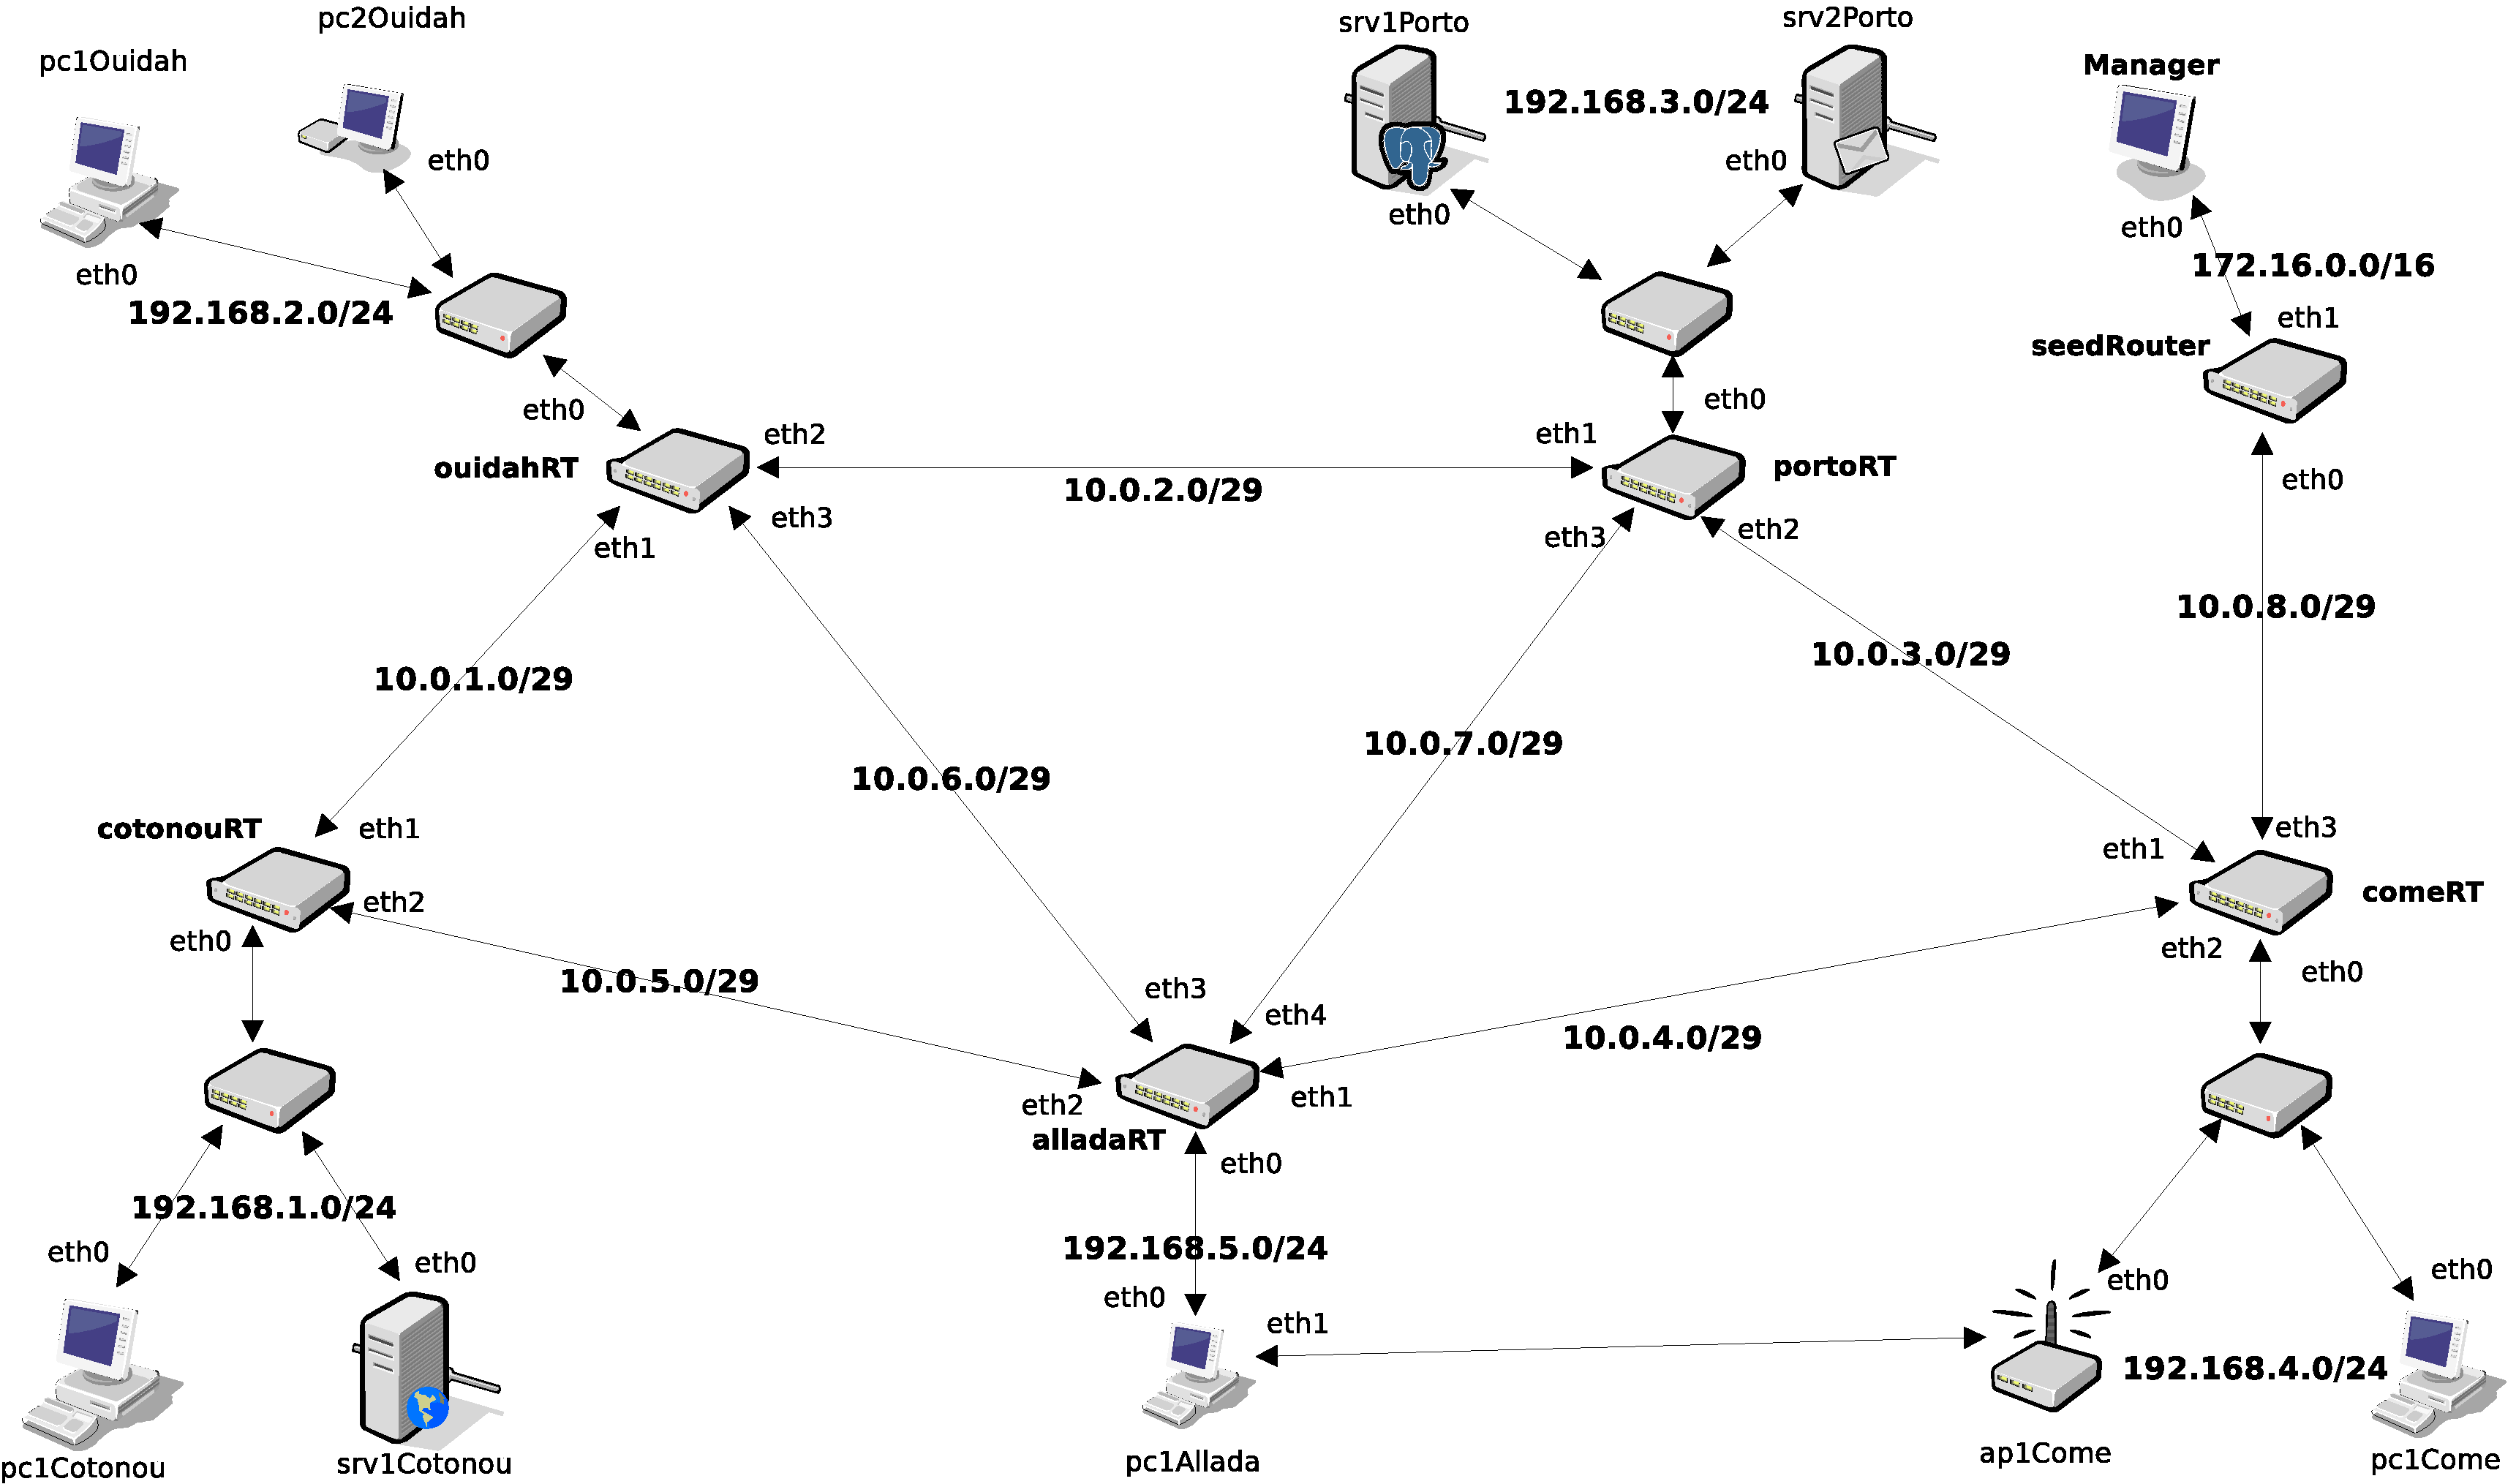
\includegraphics[scale=0.3]{images/snmp_lab.pdf}
     \caption{Modèle de réseau (crée avec NetKit) à découvrir par le seedDB} \label {fig:snmp_lab} 
        \end{center}
   \end{figure}
La figure \ref{fig:snmp_lab} (page \pageref{fig:snmp_lab}) montre le modèle de réseau crée. Ce laboratoire est constitué des équipements ayant les caractéristiques réseaux suivantes:
\begin{itemize}
\item PCs
\begin{itemize}
\item pc1Cotonou (\texttt{192.168.1.1} sur \texttt{eth0})
\item pc1Ouidah (\texttt{192.168.2.1} sur \texttt{eth0})
\item pc2Ouidah (\texttt{192.168.2.2} sur \texttt{eth0}) 
\item pc1Allada (\texttt{192.168.5.1} sur \texttt{eth0} et \texttt{192.168.4.100} sur \texttt{eth1})
\item pc1Come (\texttt{192.168.4.1} sur \texttt{eth0}) 
\end{itemize}
\item Serveurs
\begin{itemize}
\item srv1Cotonou (\texttt{192.168.1.2} sur \texttt{eth0})
\item srv1Porto (\texttt{192.168.3.1} sur \texttt{eth0}) 
\item srv2Porto (\texttt{192.168.3.2} sur \texttt{eth0})      
\end{itemize}
\item Access Point: ap1Come (\texttt{192.168.4.2} sur \texttt{eth0})
\item Routeur
\begin{itemize}
\item rtCotonou:
\begin{itemize}
\item \texttt{eth0}: \texttt{192.168.1.100}
\item \texttt{eth1}: \texttt{10.0.1.1}
\item \texttt{eth2}: \texttt{10.0.5.1}
\end{itemize}
\item rtOuidah:
\begin{itemize}
\item \texttt{eth0}: \texttt{192.168.2.100}
\item \texttt{eth1}: \texttt{10.0.1.2}
\item \texttt{eth2}: \texttt{10.0.2.2}
\item \texttt{eth3}: \texttt{10.0.6.2}
\end{itemize}
\item rtPorto:
\begin{itemize}
\item \texttt{eth0}: \texttt{192.168.3.100}
\item \texttt{eth1}: \texttt{10.0.2.3}
\item \texttt{eth2}: \texttt{10.0.3.3}
\item \texttt{eth3}: \texttt{10.0.7.3}
\end{itemize}
\item rtCome:
\begin{itemize}
\item \texttt{eth0}: \texttt{192.168.4.100}
\item \texttt{eth1}: \texttt{10.0.3.4}
\item \texttt{eth2}: \texttt{10.0.4.4}
\item \texttt{eth3}: \texttt{10.0.8.4}
\end{itemize}
\item rtAllada:
\begin{itemize}
\item \texttt{eth0}: \texttt{192.168.5.100}
\item \texttt{eth1}: \texttt{10.0.4.5}
\item \texttt{eth2}: \texttt{10.0.5.5}
\item \texttt{eth3}: \texttt{10.0.6.5}
\item \texttt{eth4}: \texttt{10.0.7.5}
\end{itemize}
\item seedRouter: 
\begin{itemize}
\item \texttt{eth0}: \texttt{10.0.8.6}
\item \texttt{eth1}: \texttt{172.16.0.6}
\end{itemize}
\end{itemize}
\end{itemize}
Le \emph{Manager} ne fait pas partie du réseau virtuel. L'adresse IP de son interface en communication avec le réseau virtuel est: \texttt{172.16.0.7}.

L'adresse \texttt{eth1} du \texttt{seedRouter} est totalement différent de celui du réseau virtuel (nous passons de la classe A à la classe B) pour éviter un conflit au niveau des adresses des interfaces \texttt{tap} et de celui du réseau virtuel de \emph{Netkit}.


Nous donnerons comme point de départ à notre algorithme, le \texttt{seedRouter}. A noter que \emph{SNMP} est déjà configuré par nos soins sur tous les équipements. Pour que depuis notre PC, nous puissions accéder au réseau virtuel à travers le \texttt{seedRouter} , il faut activer au  niveau du \texttt{seedRouter}, l'interface \texttt{tap}. 


Vu que \emph{NAV} ne supporte pas encore \emph{SNMPv3}, et que la typologie vas être découverte par \texttt{ipdevpoll} du \emph{NAV}, notre code pour plus de cohésion, implémente la classe \emph{SNMP} du \emph{NAV}, qui en fait est une extension de la classe \emph{pysnmp} (module SNMP de python).



Pour finir sur le réseau virtuel, notons que les hôtes du réseau peuvent être tout type d'équipement. Dans le cadre de cette étude nous nous sommes limités aux PCs, Switchs L2, serveurs et routeurs. Le plus important étant que l'équipement ajouté dans le réseau supporte \emph{SNMP} et soit correctement configuré.

\subsubsection{Résultats}
La classe \texttt{SeedDB} est ajouté dans le répertoire \texttt{/opt/nav-3.11.5/python/nav/seeddb}. L'appel de la classe avec les paramètres correctes donne:
\lstset{language=Python,basicstyle=\color{bookColor},basicstyle=\ttfamily,backgroundcolor=\color{White},basicstyle=\tiny} 
\begin{lstlisting}[frame=single] 
$ pwd
/opt/nav-3.11.5/python/nav/seeddb
$ sudo python seeddb.py

========================================================
=== Welcome to NAV SNMP based Network Host Discovery ===
========================================================

Enter starting router IP: 172.16.0.6
[OK] seed_router...
==============================================
==== Select SNMP version for your Network ====
==== 1 for SNMP v1                        ====
==== 2 for all versions of SNMP v2        ====
==== 3 for SNMP v3                        ====
==============================================
2
Enter community for version 2: public

Checking SNMP parameters...

[OK] SNMP parameters...
Starting device discovery

Getting all routers on the network

[OK] Routers list...

Getting all Hosts on the network

I'am affraid, looks like something went wrong with 10.0.8.6 !
===== get_local_net_address error =====
Timed out waiting for SNMP response: Manager: no response arrived before timeout


[OK] All devices list...

Setting all network Host type

[OK] Device type...

Creating bulk import file

[OK] Create bulk import file: /tmp/nav/ip_device_bulk_import_20120829013534.txt
Exiting...


\end{lstlisting} 
La classe \texttt{SeedDB} ajoute à chacun de son appel, plus de détails sur le déroulement du processus de découverte des équipements dans le fichier \texttt{/var/log/nav/autoseeddb.log} spécifié dans la classe \texttt{SeedDB}. Ce fichier journal contient beaucoup de ligne pour chaque opération: ajout dans le tableau des routeurs, regroupement des routeurs, ajout des équipements du réseau local, regroupement des équipements du réseau local, identification des types d'hôte, création du fichier d'importation. Les dernières lignes de ce fichiers peuvent donner au cas où tout c'est bien déroulé:
\lstset{language=Python,basicstyle=\color{bookColor},basicstyle=\ttfamily,backgroundcolor=\color{White},basicstyle=\tiny} 
\begin{lstlisting}[frame=single] 
$ tail -f /var/log/nav/autoseeddb.log 
[ 2012-08-29 01:35:34,900 ][ INFO     ] root - Adding line myroom:192.168.5.1:myorg:OTHER:public in file
[ 2012-08-29 01:35:34,900 ][ INFO     ] root - Adding line myroom:10.0.5.1:myorg:GW:public in file
[ 2012-08-29 01:35:34,900 ][ INFO     ] root - Adding line myroom:10.0.7.3:myorg:GW:public in file
[ 2012-08-29 01:35:34,900 ][ INFO     ] root - Adding line myroom:10.0.2.2:myorg:GW:public in file
[ 2012-08-29 01:35:34,900 ][ INFO     ] root - Adding line myroom:10.0.3.4:myorg:GW:public in file
[ 2012-08-29 01:35:34,900 ][ INFO     ] root - Closing file /tmp/nav/ip_device_bulk_import_20120829013534.txt
[ 2012-08-29 01:35:34,900 ][ INFO     ] root - Create bulk import file: /tmp/nav/ip_device_bulk_import_20120829013534.txt
[ 2012-08-29 01:35:34,900 ][ INFO     ] root - Exiting at the end of the script...
\end{lstlisting} 

Le fichier obtenu se présente comme suit:
\lstset{language=Python,basicstyle=\ttfamily,backgroundcolor=\color{fondBleu},basicstyle=\tiny} 
\begin{lstlisting}[frame=single] 
$ cat /tmp/nav/ip_device_bulk_import_20120829013534.txt
myroom:10.0.8.6:myorg:GW:public
myroom:172.16.0.7:myorg:OTHER:public
myroom:192.168.1.1:myorg:OTHER:public
myroom:192.168.1.2:myorg:OTHER:public
myroom:192.168.3.1:myorg:OTHER:public
myroom:192.168.3.2:myorg:OTHER:public
myroom:192.168.2.1:myorg:OTHER:public
myroom:192.168.2.2:myorg:OTHER:public
myroom:192.168.4.1:myorg:OTHER:public
myroom:192.168.4.2:myorg:OTHER:public
myroom:10.0.7.5:myorg:GW:public
myroom:192.168.5.1:myorg:OTHER:public
myroom:10.0.5.1:myorg:GW:public
myroom:10.0.7.3:myorg:GW:public
myroom:10.0.2.2:myorg:GW:public
myroom:10.0.3.4:myorg:GW:public
\end{lstlisting}
Les figures \ref{fig:seeddb_import_1} (page \pageref{fig:seeddb_import_1}) et \ref{fig:seeddb_import_2} (page \pageref{fig:seeddb_import_2}) montrent les résultats d'importation du fichier généré par \texttt{SeedDB} dans NAV.

\begin{figure}[H]
    \begin{center}
     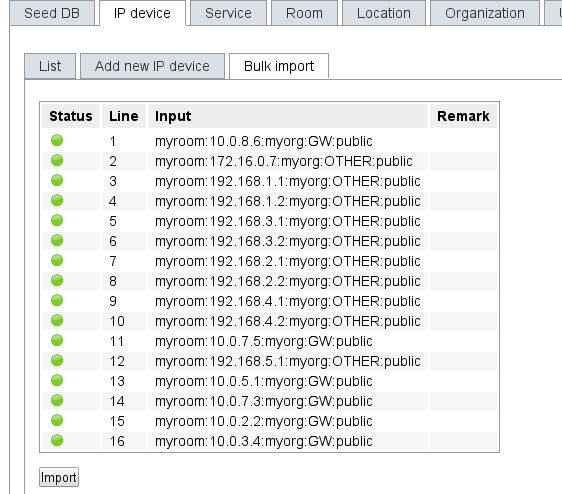
\includegraphics[scale=0.7]{images/seeddb_import.png}
     \caption{Fenêtre de confirmation de l'importation des données du fichier des équipements du réseau} \label {fig:seeddb_import_1} 
        \end{center}
   \end{figure}

\begin{figure}[H]
    \begin{center}
     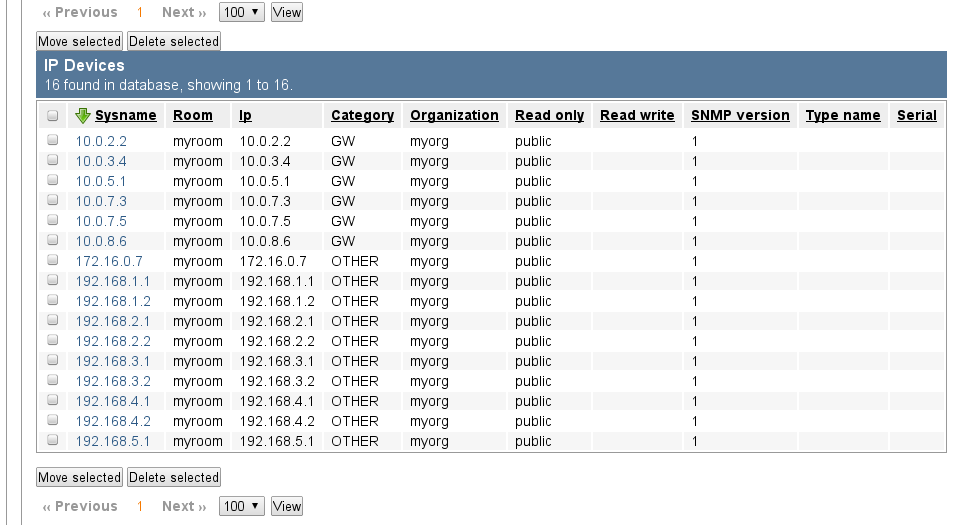
\includegraphics[scale=0.5]{images/seeddb_import_suite.png}
     \caption{Résultat de l'importation du fichier des équipements du réseau} \label {fig:seeddb_import_2} 
        \end{center}
   \end{figure}
   		
   	%Conclusion
	\conclusion
La supervision réseau est un élément capital dans le monde moderne. Elle est la clé de l'assurance de la QoS. Des esprits plus avisés en ont pris conscience très tôt, dès de début d'Internet en élaborant le protocole \emph{\gls*{sgmp}} qui deviendra très vite \emph{SNMP}.

Très bien accueilli par les constructeurs (à cause de sa \emph{simplicité}), ce protocole reste le standard actuel en matière de supervision. La version reconnue comme standard actuellement est la \emph{SNMPv3}. 

Plusieurs solutions de supervision ont été développé sur la base de \emph{SNMP}. Dans ce lot, le \emph{Network Administration Visualized (NAV)} se singularise. En effet, le NAV est une collection de solutions libres ayant déjà fait leur preuve, chacun dans son domaine. Le NAV offrent ainsi de nombreuses fonctionnalités permettant une gestion optimale du réseau. Mais comme tout projet, le NAV souffrent de quelques limites. La première limite est relative au domaine d'utilisation de la solution. NAV est d'origine universitaire et semble être limitée au monde universitaire. D'autres limites sont reconnues par les développeurs de la solution sur la feuille de route des améliorations du projet. Parmi les fonctionnalités à ajouté au NAV figurent, l'\emph{autodiscovery-wizard}. Cette fonctionnalité permettra de simplifier la première étape après l'installation du NAV: le \texttt{seed DB}. L'étape  du \texttt{seed DB} permet d'enregistrer dans la base de données du NAV, un par un ou par bloc les équipements du réseau. Ce travail peut être fastidieux lorsqu'on est dans un large réseau. 

Notre apport au NAV est l'\emph{initialisation automatique de la base de données} en s'inspirant des dernières études en matière de découverte automatique des équipements d'un réseau grâce à SNMP. Ainsi à partir d'un routeur, il est possible de connaitre tous les équipements actifs dans un réseau. Notre implémentation permet en plus de connaître tous les équipements actifs du réseau; de connaître le type de chacun d'eux et de créer un fichier prêt pour importation dans le NAV. La découverte des équipements du réseau se déroule en étapes suivantes:
\begin{enumerate}
 \item Vérification des paramètres SNMP.
 \item Découverte des équipements du réseau.
 \begin{enumerate}
  \item Découverte des routeurs.
   \begin{enumerate}
    \item Regroupement des équipements pour éviter les doublons.
   \end{enumerate}
  \item Découverte de tous les équipements actifs dans chaque réseau local.
  \begin{enumerate}
   \item Regroupement des équipements pour éviter les doublons.
  \end{enumerate}
 \end{enumerate}
 \item Découverte des types d'équipement.
 \item Création du fichier d'importation dans le NAV.
\end{enumerate}
Fini donc les ajouts manuels, avec les risque de doublons ou d'oubli. Il suffit de lancer le script avec les bons paramètres pour obtenir dans un fichier au format d'import en masse de NAV des équipements du réseau.

Ce fichier est uniquement conforme au \emph{Level 1: Minimum requirements}\footnote{\url{http://nav.uninett.no/seedessentials}} pour l'importation en masse avec NAV. Or pour pouvoir bénéficier pleinement des fonctionnalités du NAV, il faut enregistrer les donnés selon le \emph{Level 3: Take full advantage of NAV's capabilities}. Ce niveau permet la personnalisation des salles, des localisations, des organisations gérant les équipements et/ou adresses IP, etc. 

Aussi, l'import dans la base pourrait se faire sans passer par la génération d'un fichier, quoique temporaire. Notre implémentation génère un fichier qu'il faudra importer dans la base du NAV. Cette étape supplémentaire pourrait être éliminée en insérant les informations relatives aux équipements directement dans la base de données du NAV sans passé par l'interface web pour importation. 

NAV ne supporte que \emph{SNMPv1} et \emph{SNMPv2}. Dans un souci de compatibilité avec NAV, notre implémentation est basé sur la classe native \texttt{Snmp} du NAV. Cette classe est d'ailleurs utilisée par le processus du \texttt{ipdevpoll}\footnote{\url{https://nav.uninett.no/backendprocesses}} processus  de découverte de la typologie du réseau. Notre implémentation est donc tout à fait compatible avec le NAV. L'utilisation de \emph{SNMPv3} est toujours possible avec notre implémentation, mais les risques d'incompatibilité avec \texttt{ipdevpoll} nous on conduit à mettre cette option comme fonctionnalité futur.

L'essentiel des fonctionnalités du NAV n'ont pu être testé. Faute d'un ordinateur constamment allumé d'une part. D'autre part, le réseau de test est un réseau virtuel crée grâce à \emph{NetKit}. La disponibilité d'un ordinateur fonctionnant 24h/24 et d'un réseau réel  permettra de mieux observer les diverses fonctionnalités du NAV.
	
	%Biblio
	\begin{thebibliography}{9}\addcontentsline{toc}{chapter}{Bibliographie}

\bibitem{S}
  Douglas R. Mauro, Kevin J, 2005:
  \emph{Essential SNMP, Second Edition},
  O'Reilly Media, 462 p,
  \url{http://shop.oreilly.com/product/9780596008406.do}
  
\bibitem{SP}
   NGUYEN Manh Tuong.
  \emph{Les protocoles pour la gestion des réseaux Informatiques }.
  2005.
  \url{http://www2.ifi.auf.org/rapports/tpe-promo10/tipe-nguyen_manh_tuong.pdf}
  
\bibitem{AR}
   Yves Bertsch, Frederic Stmarcel.
  \emph{Administration Réseau-système SNMPv1, SNMPv2, SNMPv3 et HTTP }.
  2001.
  \url{http://2001.jres.org/actes/snmpvhttp.pdf}
  
\bibitem{SW}
   Simple Web (Aiko Pras, Ramin Sadre), Design and Analysis of Communications Systems (DACS) group, University of Twente, The Netherlands, 
  \emph{Internet Management Tutorials }.
  2012.
  \url{http://www.simpleweb.org/wiki/Internet_Management_Tutorials}

\bibitem{AT1}
Pandey, Choi, Lee and Hong.
\emph{IP Network Topology Discovery Using SNMP}. 
International Conference on Information Networking (ICOIN'09). 23 33-37 2009
  \url{http://dpnm.postech.ac.kr/papers/ICOIN/09/TopologyDiscovery_November_18.pdf}

\bibitem{AT2}
Yang Xiao.
\emph{Physical Path Tracing for IP Traffic using SNMP}. 
BBC Research White Paper WHP 188 2010

\bibitem{AT3}
Pandey, Choi, Won and Hong.
\emph{SNMP-based enterprise IP network topology discovery}. 
 International Journal of Network Management 21 (3) 169-184. 2011
 
\bibitem{AT4}
Musa Balta, Ibrahim Özçelik
\emph{The Discovery of Enterprise Network Topology Created in a Virtual
Environment with SNMPv3}. 
The Online Journal of Science and Technology (TOJSAT) Volume 2, Issue 2, 64-70, April 2012.


\bibitem{DIT}
  R. Siamwalla, R. Sharma, S. Keshav
  \emph{Discovering Internet Topologym}.
   Cornell Network Research Group, Department of Computer Science, Cornell University, Ithaca, 1988.

\bibitem{PT}  
Bierman and Jones 
\emph{Physical topology MIB}.
IETF web page, 2000
 \url{http://www.ietf.org/rfc/rfc2922.txt} 
 

\bibitem{Py}
  Mark Lutz.
  \emph{Learning Python, Fourth Edition},
  O'Reilly Media, 1214 p, 2009.
  
\bibitem{Py1}
  Mark Lutz.
  \emph{Programming.Python, Fourth Edition},
  O'Reilly Media, 1628 p, 2010.
  %\url{http://shop.oreilly.com/product/9780596008406.do}

 
\end{thebibliography}
	
  %%%% Fin du document %%%%

	%Annexes
	\appendix

\end{document}          
